%%=============================================================================
%% Methodologie
%%=============================================================================

\chapter{\IfLanguageName{dutch}{Methodologie}{Methodology}}
\label{ch:methodologie}
In dit deel wordt eerst overlopen aan welke voorwaarden software moet voldoen om te kunnen dienen als leermiddel. Vervolgens worden deze voorwaarden afgetoetst aan de gevonden software om zoo een aantal test omgevingen voor te definiëren. Hierna woorden de resultaten van de tests besproken om af te sluiten met algemeen resultaat.

%% Hoe ben je te werk gegaan? Verdeel je onderzoek in grote fasen, en
%% licht in elke fase toe welke stappen je gevolgd hebt. Verantwoord waarom je
%% op deze manier te werk gegaan bent. Je moet kunnen aantonen dat je de best
%% mogelijke manier toegepast hebt om een antwoord te vinden op de
%% onderzoeksvraag.

\section{Selectie software}
Om software te vinden die toepasbaar is om gebruikt te worden als lesmateriaal moeten er bepaalde vereisten voldaan zijn.

\begin{itemize}
    \item Kosteloos zijn; als er kosten zijn mogen deze de leer ervaring niet ten nadele komen.
    \item Uitvoerbaar op de computers van de studenten. Mag door de verschillen in besturingssystemen van studenten computers niet te veel verschillen in werking.
    \item De software moet op zichzelf of in combinatie met ander software de volledige levenscyclus van containers kunnen tonen en niet te restrictief in gebruik zijn.
    \item Niet te complex zijn om te gebruiken.
    \item Geen verwaarloosde software zijn.
\end{itemize}
    
\subsection{Algemene toepassing voorwaarden op gevonden software}
Door een klassieke VM te gebruiken om daarin te werken kunnen de problemen met de uitvoerbaarheid op het gast besturingssystemen vermeden worden en zal de ingebruikname ook binnen de VM voor alle studenten hetzelfde zijn. Dit heeft ook het voordeel dat het besturingssysteem van de VM een Linux distributie kan zijn, een voorwaarde die nodig is om veel van software te kunnen draaien. De rest van deze sectie zal iets specifieker de gevonden technologieën overlopen.

Met uitzondering van technologieën die op Cloud berusten, de repositories of volledige Cloud services, zijn alle van de gevonden technologieën gratis te gebruiken. Ook is er door het OCI een zekere mate van mudulariteit tussen de technologieën. Software mag dan zelf niet de volledige orchestration kunnen doen, zal er een zekere integratie zijn met software dit dat wel kan.

\subsection{Engines en runtimes}
Qua geschiktheid om als runtime komen Docker engine en Podman het beste uit. Docker Dankzij zijn populariteit en veelvuldigheid. Hiermee is er ook veel onlinehulp te vinden voor het gebruik van Docker. Podman ’s vriendelijkheid als leermiddel is deels te danken doordat het zich opstelt als een duidelijk alternatief voor Docker op Linux distributies. De directe hulp een uitleg om met Podman te werken mag dan al iets minder zijn, die werking van Podman zou kort beschreven kunnen worden als hetzelfde als dat van Docker qua commando’s met een ingebouwde ondersteuning voor pods van meerdere containers.  Verder zou Containerd ook nog een alternatief kunnen zijn maar dan nipt op de rand van de complexiteit, zeker in vergelijking met Podman en Docker. Tabel \ref{tab:Engines} toont van deze en de andere grotere gevonden engines, runtimes of containers hun restricties en complexiteiten. 

Om zelf te werken met Linux containers is te complex om een goede introductie tot containers te zijn. Windows containers zijn enkel mogelijk op bepaalde distributie van Windows en berusten verder op de Docker engine voor de uitvoering, hierdoor is de extra stap om met deze containers te werken ten opzichte van Docker geen meerwaarde als inleiding. Een gebrek aan uitleg voor het gebruik van cri-o doet twijfelen aan de geschiktheid voor Cri-o als runtime.  Het unieke verkooppunt van Kata containers, de mogelijkheid om ook VM’s als containers te draaien is een stap in complexiteit te ver om een goede inleiding to container virtualisatie te zijn.  De rest van de gevonden runtimes zijn te klein of al te lang zonder ondersteuning om met zekerheid te kunnen zeggen dat ze relevant zullen blijven voor containers en verwante technologieën. 

\begin{center}
    \begin{table}
    \begin{tabular}{ m{3.5cm} || m{1cm} | m{3.3cm} | m{4.5cm} }
        Engine/container & Gratis & Besturingssysteem restricties & Bijkomende complexiteit t.o.v. Docker \\ 
        \hline
        Docker & ja & geen &  \\  
        \hline
        Containerd & ja & De meeste Linux distributies & Werkt voor sturing met Go programma’s \\
        \hline 
        Linuxcontainers & ja & Linux & Zelf configureren via het besturingssysteem \\
        \hline
        Cri-o & ja & De meeste Linux distributies & Enkel voor werking met Kubernetes \\
        \hline
        Podman & ja & De meeste Linux distributies & Veel overgenomen van Docker + Ingebouwde pods \\
        \hline
        Windows containers & ja & Windows, exlusief Home Edities & Werkt enkel met Docker/ Niet van toepassing \\
        \hline
        PouchContainer & ja & Ubuntu of CentOS & Slechte documentatie \\
        \hline
        Kata containers & ja & De meeste Linux distributies & Extra Configuratie, nood aan Containerd of Cri-o voor uitvoering \\
    \end{tabular}
    \label{tab:Engines}
    \caption[Overzicht Runtimes en containers]{Een overzicht van gevonden runtimes of containers met hun restricties en toegevoegde complexiteit.}
    \end{table}
\end{center}

\subsection{Orchestration}
Docker compose is een uitbreiding van de Docker engine en is daarmee ook gratis en heeft dezelfde vereisten als Docker, het wordt zelf standaard geïnstalleerd met de Docker desktop applicatie. Kubernetes en Nomad zijn verder nog twee softwarepakketten die goed zouden kunnen zijn om met te leren. Kubernetes is de meest gebruikte orchestration software en is daarmee zoals Docker voorzien van veel online tutorial. Het is open source en kan met veel van de runtimes werken. Voor het leren werken met Kubernetes is er ook Minikube die je lokaal in staat stel met Kubernetes te werken. Nomad is orchestration software die lijkt op Kubernetes maar toch zichzelf wilt onderscheiden van Kubernetes door meer dan alleen containers te kunnen beheren. Tabel \ref{tab:Ochestration} toont voor de ochetration software een overzicht.
\begin{center}
    \begin{table}
        \begin{tabular}{ m{3cm} || m{1.5cm} | m{3.3cm} | m{4.5cm} }
            Software & Gratis & Besturingssysteem restricties & Bijkomende complexiteit t.o.v. Docker \\ 
            \hline
            Docker Compose & ja & geen &  \\  
            \hline
            Docker Swarm & ja & geen & \\
            \hline 
            Kubernetes & ja & geen & Minikube als middleware voor lokale uitvoering \\
            \hline
            OpenShift & 30-day trail & Red Hat Besturingsystemen & Zelf Datacenter opzetten of Cloud gebruiken \\
            \hline
            Nomad & ja & geen & Eigen configuratie taal \\
            \hline
            Apache Mesos & ja & geen & Met binairy of zelf lokaal builden.  \\
            \hline 
            DC/OS & ja & DC/OS & Zelf datacenter opzetten \\
        \end{tabular}
        \label{tab:Ochestration}
        \caption[Overzicht ochestration]{Een overzicht van gevonden Ochestration software met hun restricties en toegevoegde complexiteit.}
    \end{table}
\end{center}

De specifieke besturingen systemen orchestration DC/OS of een volledige datacenter opzetten met Apache Mesos zijn te complex om een duidelijke introductie te zijn tot container virtualisatie.  Openshift is een te commercieel en bedrijfsgericht product om makkelijk in gebruikt te nemen als student. En tenslotte is er nog de Docker swarm die zelf aan populariteit verliest ten opzichte van Kubernetes als software voor orchestration.



\subsection{Image repositories}
Met dat het OCI en hun container image geslaagd is in de standaardisatie container images zijn repositories vrij met elkaar te verwisselen. De Docker hub en de GitHub container registry zijn de meest geschikt om door een student als image repository te gebruiken.  Docker hub doordat het bijna overal als standaard gebruikt wordt en de GitHub omdat een student wellicht al een GitHub account hebben. Ook de kostenstructuur van de twee is te vergelijken met gratis publieke images en betaling vanaf een bepaalde drempel voor private images. Tijden het schrijven van deze thesis is de GitHub container registry wel no in een bètafase waardoor het volledig gebruik gratis is. een overzicht van deze twee en Gitlab staat in tabel \ref{tab:repositories}.

\begin{center}
    \begin{table}
        \begin{tabular}{ m{3.5cm} || m{2cm} | m{3.3cm} | m{4.5cm} }
            Repository & Gratis Account & Limiet gratis privé images & Overdracht limiet \\ 
            \hline
            Docker hub & ja & 1 image & 100 per 6 uur anoniem en 200 per 6 uur ingelogd
             \\  
            \hline
            GitHub Container Registry & ja & 500 mb* & Niet gespecifieerd \\
            \hline 
            Gitlab Container Registry & 30-day trail & Niet gespecifieerd & Niet gespecifieerd \\
            \multicolumn{4}{c}{ } \\
            \multicolumn{4}{l}{*In beta waren geen limieten van toepassing, het zal de Github Packages limieten delen.} \\
        \end{tabular}
        \label{tab:repositories}
        \caption[Overzicht image repositories]{Een overzicht van gevonden image repositories met hun limieten voor gratis accounts.}
    \end{table}
\end{center}

\subsection{Cloud hosting en servces}
Cloud hosting services kunnen een optie zijn maar afhankelijk van de host kan het dat een free trial niet toegang geeft tot alle tools die nodig zijn of is het moeilijk om gratis krediet te krijgen. Zo geeft Amazon geen gratis krediet meer of vraagt Google voor een creditcard.  Verder zal het maken van een image eerst lokaal moeten gebeuren waarvoor een lokale runtime nodig is. Hierdoor kan er even goed in eerste instantie lokaal verder gewerkt worden.

\section{Software Tests}
Wegens de modulariteit gecreëerd door het OCI zullen eerst de runtimes uitgeprobeerd worden om daarna te kijken naar de mogelijkheden van de runtimes om te werken met toegewijde orchestration software.

\subsection{Runtimes}
Voor deze is het voornaamste belang dat containers kunne gemaakt gedraaid en gestopt worden door middel van de runtime ook moet het persisteren van data naar een volume en het pullen van een image mogelijk zijn.

\paragraph{Docker Desktop}
De Docker desktop een applicatie voor Windows en Mac die Dockers engine combineert met Docker-compose, lokale Kubernetes, een dashboard en een eenvoudige verbinding met de Docker hub. Wegens de volledigheid van deze bundel zal dit als eerste uitgeprobeerd worden. Doordat de desktop applicatie niet voor Linux bestaat is deze echter niet volledig toepasbaar voor alle studenten. Een Linux gebruiker zou de delen apart moeten installeren. Dit is ook de software die direct op een laptop zal worden uitgevoerd en niet in een VM. Ook zal dit gebruikt worden als een baseline voor vergelijkingen. 

\paragraph{Fedora Podman}
Een eerste VM waarin het meest beloftevolle alternatief wordt getest is Fedora workstation instantie. Deels omdat Fedora al gebruikt wordt tijdens het vak besturingssystemen en omdat het ook standaard met een Firefox webbrowser komt waarmee het gemakkelijk is om te testen of een webservice gebaseerde container draait.

\paragraph{Ubuntu Podman}
Om Podman ook uit te proberen op een ander besturingssysteem dan Fedora zal ook eens geprobeerd worden of dat het lukt om Podman te installeren op een Ubuntu distributie.

\subsection{Orchestration}
Voor orchestration moet het mogelijk zijn om een job of taak op basis van containers te maken, aan te passen en te stoppen. En ook om iets complexer dan een enkele container service te draaien.

\paragraph{Kubernetes gebundeld met Docker desktop}
De Docker desktop applicatie komt met de mogelijkheid om een lokale Kubernetes instantie te starten. Het lijkt dus interessant om Deze ook eens te testen.

\paragraph{Podman met Minikube voor Kubernetes}
Om te testen of dat het ook mogelijk is om met Podman als runtime te werken voor Kubernetes zal er ook geprobeerd worden om een Minikube instantie werkende met Podman op te zetten en gebruiken.

\paragraph{Docker engine en Nomad}
In tegenstelling tot Kubernetes en Minikube die meer vrijheid heeft voor de achterliggende runtime heeft Nomad op dit moment enkel ondersteuning voor de Docker engine om mee te werken voor het draaien van een containers. Dus voor het uitproberen van Nomad moet er met een Docker engine gewerkt worden.

\section{Resultaten software Tests}
In dit deel worden de resultaten en ondervindingen van het werken met de eerder opgestelde software test scenario’s overlopen. 

\subsection{Docker Desktop} \label{DockerDesktop}
Het eerste dat uitgeprobeerd werd is de Docker desktop geïnstalleerd als applicatie op een laptop met 8 GB ram geheugen.

\paragraph{Installatie en set-up}
Het werken met Docker desktop direct geïnstalleerd op een Windows systeem moet er eerst het Windows Subsysteem voor Linux ingeschakeld worden. Docker verwijst hiervoor naar de help pagina’s van Microsoft. Hiervoor werden de manuele instructies van Microsoft \footnote{\url{https://docs.microsoft.com/en-us/windows/wsl/install-win10}} gevolgd om tot en met het opzetten van WSL2 als default uit te voeren. Het enigste dat hier wat specifieke aandacht vereist ten opzichte van de beschreven stappen is het controleren of dat de Windows versie geschikt is voor WSL.

Hierna werd de installer van Docker desktop uitvoeren, dit heeft een optie om WSL voor de gebruiker voor te bereiden maar omdat dit reeds gedaan was is er niet kunnen getest worden of dat dit het volledig ennablen van WSL doet of enkel verantwoordelijk is voor het instellen van een Linux distributie in WSL waarmee de containers zullen worden uitgevoerd.

\paragraph{Ingebruikname}
Bij het eerste keer opstarten van de desktop applicatie staart het met een korte tutorial die enkel het pullen builden en uitvoeren van een eenvoudige container behandelt, dit deels op een zeer korte introductie te zijn en te testen of dat de installatie gelukt is. Eveneens is het opstarten van de desktop applicatie de trigger om de backend die alles effectief draait ook te starten.

\begin{lstlisting}[caption=inhoud van de Dockerfile,label=lst:Dockerfile]
FROM node:12-alpine
RUN apk add --no-cache python g++ make
WORKDIR /app
COPY package.json yarn.lock ./
RUN yarn install --production
COPY . .
CMD ["node", "src/index.js"]
\end{lstlisting}

Vervolgens werd een uitgebreide tutorial van Docker gevolgd\footnote{\url{https://docs.docker.com/get-started/02_our_app/}}. Dit is begonnen met het kopiëren van een kleine todo-list webapplicatie gemaakt met node, gehost op GitHub\footnote{\url{https://github.com/docker/getting-started/tree/master/app}}. Voor het builden van de container wordt een dockerfile gebruikt, te zien in listing \ref{lst:Dockerfile}. Door dit op te slaan in de root van de webapplicatie kan volgend commando uitgevoerd worden in deze map voor het builden van de container.
\begin{verbatim}
docker build -t getting-started .
\end{verbatim}
Met dit commando wordt op basis van de dockerfile in de lokale map een image gemaakt en krijgt deze de tag “getting started”. Via de desktopapplicatie, afgebeeld in figuur\ref{fig:Dockerdesktop}, of het commando `docker image ls' of `docker images` wordt een lijst van lokale images getoond waaronder de aangemaakte getting started image.
\begin{figure}[h]
    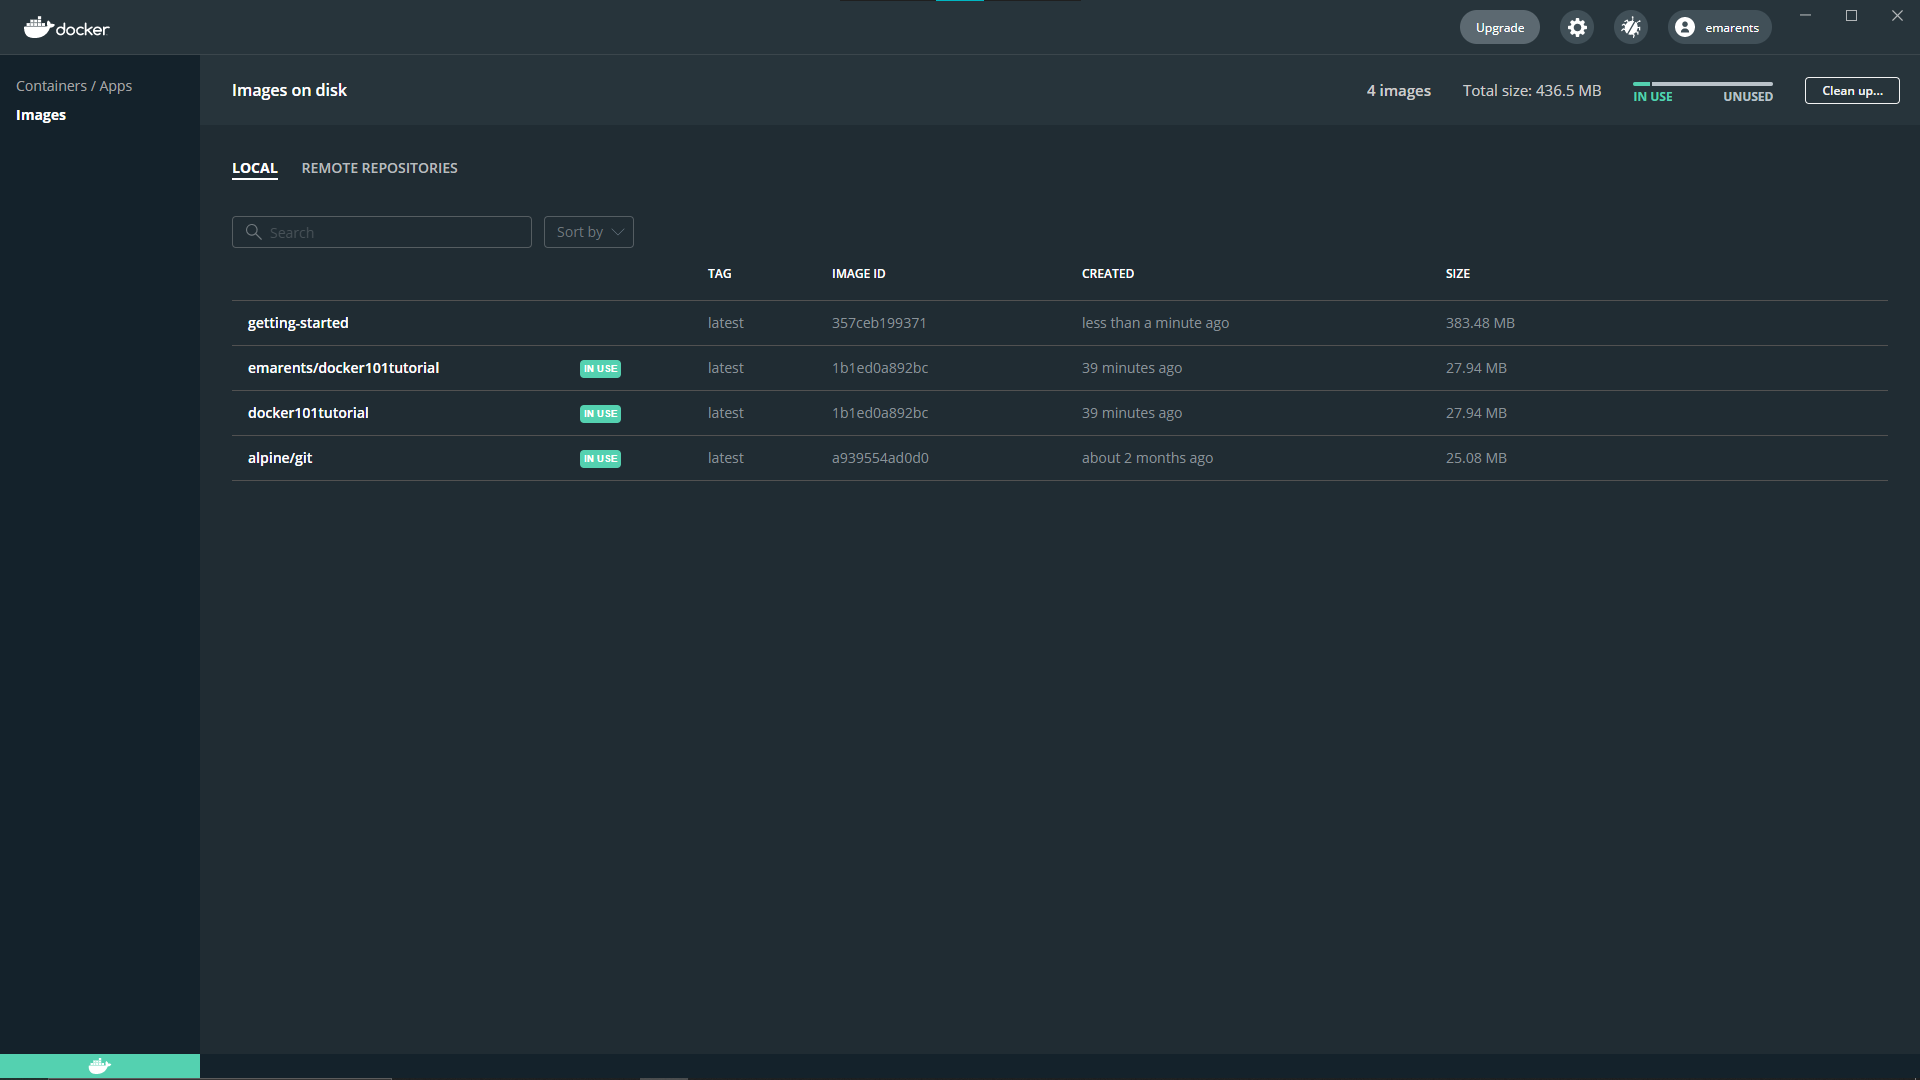
\includegraphics[width=\linewidth]{img/dockerImg.png}
    \label{fig:Dockerdesktop}
    \caption[De Docker desktop applicatie]{De Docker desktop applicatie, dit deel toont alle lokaal bewaarde images}
    \centering
\end{figure}
\begin{verbatim}
docker run -dp 3000:3000 getting-started
\end{verbatim}
Met commando wordt deze aangemaakte container uitgevoerd. ‘-p’ 3000:3000 stelt de port in zodat de webapplicatie via localhost:3000 bereikt kan worden. ‘-d’ voert de container detached uit waardoor het huidig actieve CLI niet vast wordt gehangen aan de opgestarte container.

Vervolgens werd in de bronbestanden van de todo applicatie de placeholder tekst van de applicatie te verander. Vervolgens werd de container met deze aangepaste waarde opnieuw gebuild. Vooraleer de nieuwe container met hetzelfde commando kan worden gestart moet de oude worden gestopt. Dit is mogelijk via de desktop applicatie of via CLI. Voor CLI moet ‘docker ps’ uitgevoerd worden om een lijst te krijgen van draaiende containers. In deze lijst van containers krijgt elke Container een ID. met deze ID kan de container gestopt en verwijderd worden.
Het stoppen gebeurt met:
\begin{verbatim}
docker stop <container-id>
\end{verbatim}
En het verwijderen met:
\begin{verbatim}
docker rm <container-id>
\end{verbatim}
Door bij docker rm de -f vlag toe te voegen zal een container geforceerd gestopt worden zonder manueel te moeten stoppen. Ook is het mogelijk om de container ID te vervangen met  de automatisme gegeneerde naam die Docker toekent aan een draaiende container.
Na het stoppen kan de nieuwe image met commando terug op dezelfde manier gestart worden.
\begin{verbatim}
docker run -dp 3000:3000 getting-started
\end{verbatim}
Vervolgens werd de container gepushed naar de Docker hub. Hiervoor moet er eerst een account op de Docker hub aangemaakt worden. En moet er voor dit account een nieuwe repository aangemaakt worden. Hier werd dezelfde naam getting-started gebruikt en was de repository publiek. Om de lokale image te kunnen pushen moet de lokale Docker instantie ingelogd zijn dit gebeurt via volgend commando:
\begin{verbatim}
docker login -u USER-NAME
\end{verbatim}
Om juist de container te pushen naar je eigen repository moet vervolgen de image een nieuwe tag krijgen die je gebruikersnaam specificeert hiermee krijgt de oude getting started nu de tag die verwijst naar je gebruiker en de repository naam.
\begin{verbatim}
docker tag getting-started USER-NAME/getting-started
\end{verbatim}
Hierna kan de image naar de repository worden gepushed.
\begin{verbatim}
docker push USER-NAME/getting-started
\end{verbatim}
Op dit moment verliest de todo lijst in de applicatie nog alle gegevens wanneer de container word verwijdert dus moet er een volume gebruikt worden om de inhoud op te slaan. Hiervoor moet er eerst in Docker een volume worden aangemaakt:
\begin{verbatim}
docker volume create todo-db
\end{verbatim}
Vervolgens kan de applicatie weer opgestart worden met docker run maar deze keer met een parameter voor de te gebruiken volume:
\begin{verbatim}
docker run -dp 3000:3000 -v todo-db:/etc/todos getting-started
\end{verbatim}
Als na het invullen van item in de todo applicatie de container verwijdert word zal bij het opstarten van de container met dezelfde commando de opgeslagen inhoud worden hergebruikt.

De gebruikte node.js applicatie werk standaard met een SQLite database waarbij alles weggeschreven wordt naar een bestand. Dit bestand is wat er bewaard wordt in de volume om zo hergebruikt te worden. Deze applicatie kan ook met een externe SQL-databank werken. Dit kan gedaan worden via containers.

De eerste manier is door manueel zelf de containers te verbinden over het netwerk. Hiervoor moet er eerst een netwerk aangemaakt worden in Docker.
\begin{verbatim}
docker network create todo-app
\end{verbatim}
Vervolgens wordt een MySQL databank container gemaakt op dit netwerk. Hiervoor werd volgende commando gebruikt in Windows powershell:
\begin{lstlisting}
docker run -d `
    --network todo-app --network-alias mysql `
    -v todo-mysql-data:/var/lib/mysql `
    -e MYSQL_ROOT_PASSWORD=secret `
    -e MYSQL_DATABASE=todos `
    mysql:5.7
\end{lstlisting}
Dit commando maakt een container van mysql:5.7 aan. De image die gebruikt wordt is de MySQL container versie 5.7 zoal deze te vinden is op de Docker Hub. De container wordt toegevoegd aan het netwerk en krijgt een alias. Het heeft ook een toewijzing voor de volume die gebruikt moet worden. De parameters bij de -e vlaggen zijn environment variabelen die de MySQL instantie configureren. Door middel van volgend commando is het mogelijk om de CLI van de SQL-server te bereiken.

\begin{verbatim}
docker exec -it <mysql-container-id> mysql -u root -p
\end{verbatim}
Om te achterhalen hoe dat deze MySQL server terug te vinden is binnen het aangemaakte todo-app netwerk stelt Docker voor om binnen het netwerk een nicolaka/netshoot image te runnen en te gebruiken.
\begin{verbatim}
docker run -it --network todo-app nicolaka/netshoot
\end{verbatim}
Door in de interface van de netshoot dig mysql uit te voeren kan gekeken worden of dat het gebruikte netwerk alias bij het opstarten van de container effectief in het netwerk zit. Door volgend commando uit te voeren in de root folder van de todo app zal een nieuwe container en gestart worden hierbij wordt de door de node 12-alpine image te gebruiken code en start commando's toegevoegd.

\begin{lstlisting}
docker run -dp 3000:3000 `
    -w /app -v "$(pwd):/app" `
    --network todo-app `
    -e MYSQL_HOST=mysql `
    -e MYSQL_USER=root `
    -e MYSQL_PASSWORD=secret `
    -e MYSQL_DB=todos `
    node:12-alpine `
    sh -c "yarn install && yarn run dev"
\end{lstlisting}
Eens de container gestart is kunnen de log berichten van de containers opgevraagd worden of via hetzelfde commando als eerder . De MySQL server aangesproken worden. Afbeelding \ref{fig:powershellsql} toont hoe in powershell de inhoud van de SQL databank opgehaald werd.
\begin{figure}[h]
    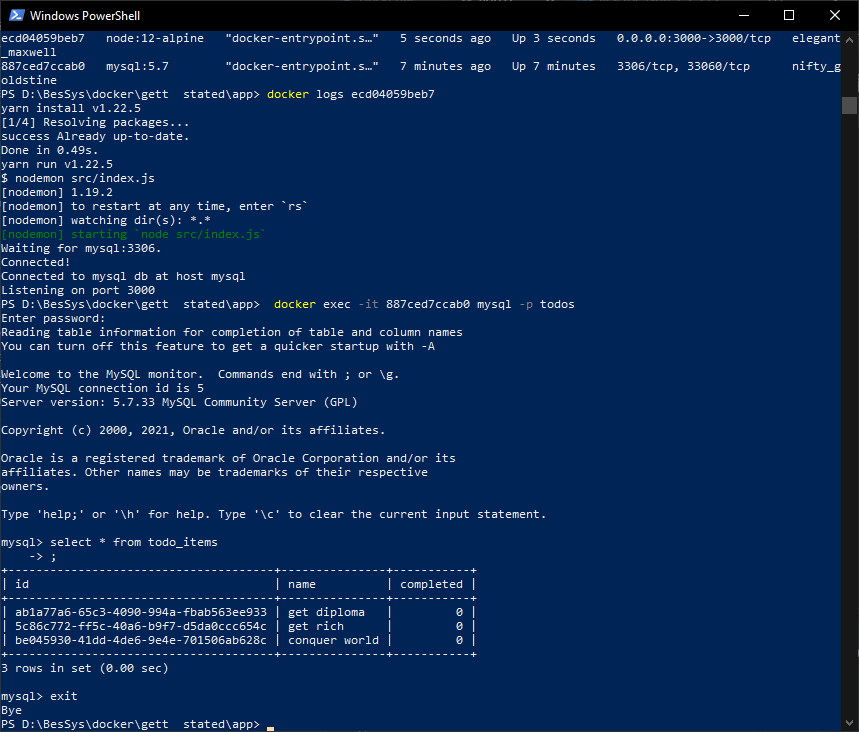
\includegraphics[width=\linewidth]{img/sqlquery.png}
    \label{fig:powershellsql}
    \caption[Het aanspreken van een SQL server binnen een container]{Met docker is er in powershell ingelogd op de SQL server die in een container staat om zo de inhoud op te halen.}
    \centering
\end{figure}

Omdat het veel stappen zijn om op deze manier een applicatie te starten is er ook Docker compose. Bij Docker compose wordt alle configuratie gedefinieerd in een yml bestand die vervolgens met compose tot het builden en verbinden van de nodige containers leidt. De inhoud van het Yyml bestand dat in voor deze applicatie gebruikt werd staat in listing \ref{lst:Composefile}.

\begin{lstlisting}[caption=inhoud van de docker-compose.yml,label=lst:Composefile]
version: "3.7"

services:
    app:
        image: node:12-alpine
        command: sh -c "yarn install && yarn run dev"
        ports:
            - 3000:3000
        working_dir: /app
        volumes:
            - ./:/app
        environment:
            MYSQL_HOST: mysql
            MYSQL_USER: root
            MYSQL_PASSWORD: secret
            MYSQL_DB: todos

    mysql:
        image: mysql:5.7
        volumes:
            - todo-mysql-data:/var/lib/mysql
        environment: 
            MYSQL_ROOT_PASSWORD: secret
        MYSQL_DATABASE: todos

volumes:
todo-mysql-data:
\end{lstlisting}
Hierbij worden voor de twee container services gedefinieerd gebaseerd op de base images die elk moet gebruiken en de environment variabelen. Ook hier wordt de node:12-alpine image lokaal gevuld met de te gebruiken inhoud. Voor het opstarten van de applicatie moet volgend commando worden uitgevoerd in de root map met het docker-compose.yml bestand.
\begin{verbatim}
docker-compose up -d
\end{verbatim}
Om het achteraf weer te stoppen kan op dezelfde plaats volgend commando uitgevoerd worden
\begin{verbatim}
docker-compose down 
\end{verbatim}
\paragraph{Ervaring}
Docker’s gebruik is eenvoudig en is ook veel over te vinden online bij eventuele problemen.  De dokker desktop geeft een grafische interface voor het beheren van draaiende containers en images, maar dit is ook allemaal mogelijk via CLI. Met de voorwaarde hier dat bij het overnemen van commando’s deze soms over meerdere regels gespreid zijn en dus dat de commando prompt van Windows niet voldoende is en overgeschakeld moet worden naar powershell.  De desktop interface maakt het wel gemakkelijk om te beheren of dat je lokale Docker instantie draait waardoor het perfect mogelijk is om het geïnstalleerd te hebben staan en buiten gebruik niet door beïnvloed worden. Het starten en stoppen van Docker in een Linux omgeving is te doen via het proces beheer van Linux zelf.  De configuratie bestanden voor containers zijn geschreven in YAML en Visual studio code heeft zelf extensie om specifiek de Docker bestanden te ondersteunen.

\subsection{Fedora Podman}
Dit werd uitgevoerd in een VM met 4 GB ram en 20 gb harde schijfruimte
\paragraph{Installatie en set-up}
Bij de verse installatie van een Fedora workstation versie 53 was Podman al inbegrepen en was er geen nood om hem te installeren.

\paragraph{Ingebruikname}
Voor het testen van het werken met Podman werden dezelfde stappen en begin bestanden gebruikt als in sectie \ref{DockerDesktop}. Dezelfde todo applicatie werd eerst lokaal gekopieerd en voorzien van een docker-/containerfile als in listing \ref{lst:Dockerfile}.

Voor het builden van de image heeft Podman het volgende commando, het uitvoeren word getoont in figuur \ref{fig:podmanbuild}.
\begin{figure}[h]
    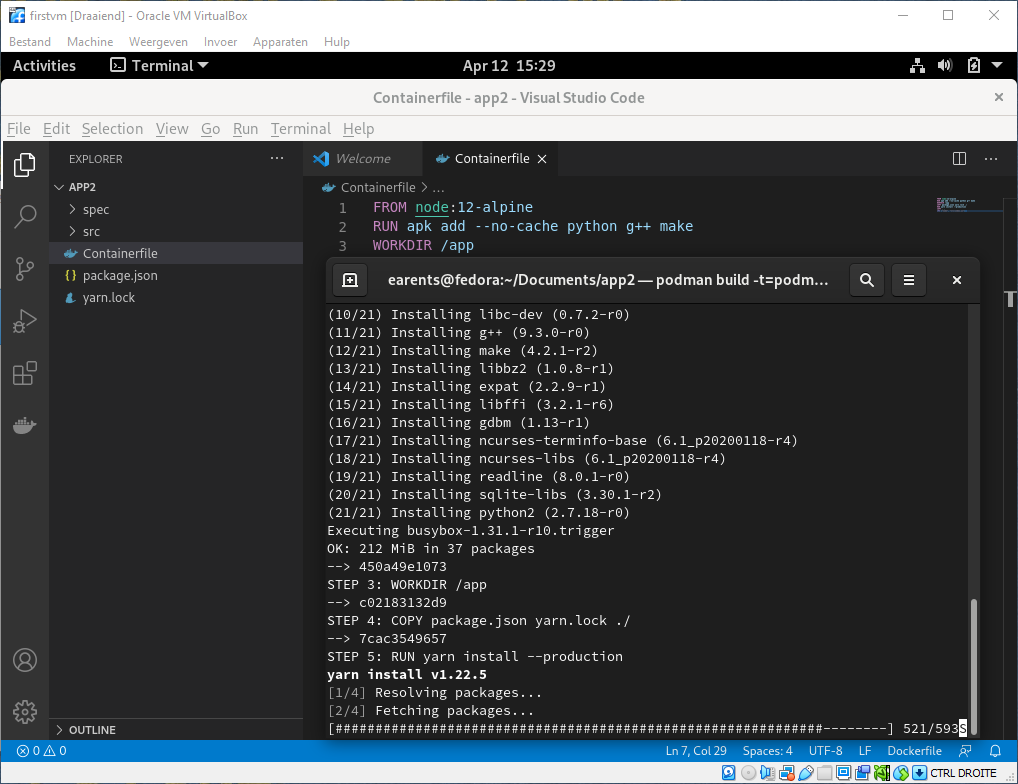
\includegraphics[width=\linewidth]{img/podmanbuild.png}
    \label{fig:podmanbuild}
    \caption[Met podman een containerfile builden]{Hier maakt Podman met het inhoudelijk zelfde docker-/containerfile as Docker een image}
    \centering
\end{figure}
\begin{verbatim}
Podman build -t getting-started .
\end{verbatim}
 
Gelijkaardig vraag je de images op met `podman images ls' of `podman images'. Ook het achterhalen van actieve containers gebeurt analoog met `podman ps'.

Vervolgens kan de container worden gestart met volgend comando en ook te zien in figuur \ref{fig:podmanrun}. 
\begin{figure}[h]
    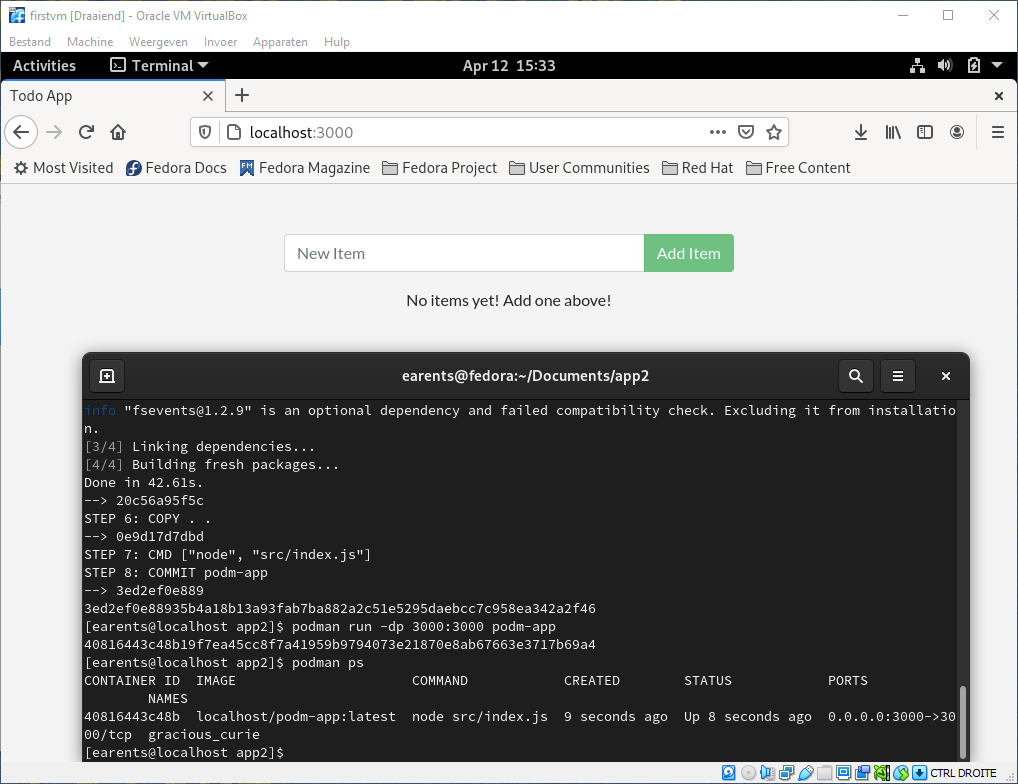
\includegraphics[width=\linewidth]{img/podmanrun.png}
    \label{fig:podmanrun}
    \caption[Podman die een web ap uitvoert]{hier is via command line de aangemaakte container gestart en wort deze op de achtergrond getoont in een webbrowser}
    \centering
\end{figure}
\begin{verbatim}
podman run -dp 3000:3000 getting-started
\end{verbatim}
het stoppen en verwijderen is ook analoog aan Docker en heeft ook de mogelijkheid om te kiezen tussen de ID of de gegenereerde instantie naam. En eventuele force vlag bij het verwijderen.
\begin{verbatim}
Podman stop <container-id>
Podman rm <container-id>
\end{verbatim}
Met volumes is er ook geen verschil, eerst het definiëren van een volume met Podman
\begin{verbatim}
Podman volume create todo-db
\end{verbatim}
En vervolgens de volume verbinden met de container bij het opstarten
\begin{verbatim}
Podman run -dp 3000:3000 -v todo-db:/etc/todos getting-started
\end{verbatim}
De verschillen van Podman met Docker komen enkel aan het ligt bij het werken met meerdere verbonden containers. Hiervoor moet er eerst een pod aangemaakt worden:
\begin{verbatim}
Podman pod create app
\end{verbatim}
Een pod krijgt bij creatie een interne container die ervoor zorgt dat de pod gedefinieerd blijf zo kan de pod gevonden worden met ‘podman pod ps’.

Bij het starten van een container is het mogelijk om een pod me te geven. Op analoge wijze als het netwerk bij Docker is geprobeerd om een MySQL instantie en de todo app aan de pod toe te kennen. Echter het effectief verbinden binnen in de pod lukte niet.
\begin{lstlisting}
docker run -d \
    --pod=app \
    -v todo-mysql-data:/var/lib/mysql \
    -e MYSQL_ROOT_PASSWORD=secret \
    -e MYSQL_DATABASE=todos \
    mysql:5.7
\end{lstlisting}

Er bestaat ook een project om Docker compose na te bootsen voor Podman genaamd Podman Compose\footnote{\url{https://GitHub.com/containers/Podman-compose}}.Door het zelfde docker-compose.yml bestand te gebruiken als in listing \ref{lst:Composefile} zal Podman compose een pod aanmaken en daaraan de containers toevoegen. 

\begin{verbatim}
podman-compose up
\end{verbatim}
Via pods ps is te zien dat de pod aangemaakt is maar de ingestelde localhost poort 3000 zoals bij Docker werkt niet. Na zonder succes te zoeken naar een manier om de interne poorten van de pod aan te spreken is dit deel beëindigd zonder te kunnen testen of dat de Podman compose of de pods werkten.

\paragraph{Ervaring}
Het werken met Docker en Podman voor eenvoudige containers te draaien lijkt sterk op elkaar, veel commando’s zijn hetzelfde en geven ook een gelijkaardig resultaat. Doordat het standaard met Fedora gebundeld is was de installatie geen probleem. Ook moet voor het te kunnen gebruiker niet zelf de lokale Podman runtime starten vooraleer je deze kan gebruiken. Echter het werken met de pods van Podman is moeilijker dan met de eenvoudige verbinding die je met Docker kan leggen.

\subsection{Ubuntu Podman}
Dit werd uitgevoerd op een VM met 4gb ram en 30 GB geheugen ruimte. Initieel was die intentie om ook hier Podman een op uit te oefenen.

\paragraph{Installatie en set-up}
Na een basis installatie van Ubuntu LTS 20.4 is er initieel geprobeerd om een installatie te doen van Podman. Volgens de help pagina’s van Podman is het mogelijk op Podman te draaien op Ubuntu. Bij het instaleren op de manieren uitgelegd is er nooit succesvol een installatie gebeurt. Na een tijd tevergeefs te zoeken naar oorzaken is er overschakelt naar het uitproberen van een ander alternatief, namelijk Containerd.
Door lokaal Golang te hebben moet het mogelijk zijn om via Containerd te werken voor container runtime. Ook hier voor het effectief installeren van Golang ondervond ik problemen.  Eens Golang geïnstalleerd lukte het echter niet om Containerd uit te voeren.

\paragraph{Ervaring}
Het is dus niet gelukt om zowel Podman als Containerd uit te voeren op Ubuntu. Voor het installeren van Podman kan het probleem zijn dat ten tijde van het proberen de repositories die Ubuntu aanreikte niet voorzien van de nodige bestanden. Voor Containerd zal het probleem liggen tussen gelijkaardige installatie problemen voor Golang. Dit gekoppeld met een tekort aan ervaring met Go heeft ervoor gezorgd dat ook Containerd niet lukte om uit te voeren.

\subsection{Kubernetes gebundeld met Docker desktop}
Dit werd opnieuw uitgevoerd aan de hand van de desktop installatie direct op de laptop. Voor de effectieve uitvoering van Kubernetes werd er gekeken naar het gebruik van GitHub als repository voor images.
\paragraph{Installatie en set-up}
Een volwaardige instantie van Kubernetes is gebundeld met de Docker desktop applicatie. Dit betekent wel dat het op Linux systemen niet gelijkaardig zal zijn.
Voor de GitHub Container Registry is het ten tijde van dit onderzoek nodig om manueel deel te nemen aan de beta versie. Ook stelt GitHub voor om een access token te maken voor het inloggen en verbinden met je container registry.

\paragraph{Ingebruikname}
Om een lokale image te kunnen pushen naar een eigen repository en niet bij het uitvoeren van de push te pushen naar de oorspronkelijke repository van de base image moet de lokale image getagd worden met een verwijzing naar de gewenste repository op de GitHub container registry:
\begin{verbatim}
Docker tag getting-started ghcr.io/username/getting-started:1.0
\end{verbatim}

Deze zal in de image lijst een kopie maken van de getting-started image en als tag voor versie 1.0 instellen. Om deze effectief te up te loaden moet het nog manueel worden gepushed.
\begin{verbatim}
Docker Push ghcr.io/username/getting-started:1.0
\end{verbatim}

Hiermee wordt de container image bewaard in het packages gedeelte van GitHub. De nodige package wordt automatisch aangemaakt en is ten tijde van de bèta versie initieel privé.

Voor het pullen van images zal de naam eerst gezocht worden op de Docker hub. Het is nodig, zelfs wanneer ingelogd op GitHub, om manueel de volledige adressering te specifiëren:
\begin{verbatim}
Docker pull ghcr.io/username/getting-started:1.0
\end{verbatim}


De gebundelde Kubernetes van de Docker desktop lukte niet om te gebruiken. Bij het opstarten van Kubernetes via de desktop worden alle nodige onderdelen geïmporteerd en opgestart in hun eigen containers. Kubernetes is niet volledig kunnen starten. Windows task manager gaf aan dat de laptops processor en ram geheugen overbelast werden. Verder toonde de interface van Docker desktop hoe bepaalde containers voor de werking opstartte, afgebroken werden en weer opgestart werden.

\paragraph{Ervaring}
Het werken met de GitHub Container Registry loopt vlot het voornaamste jammerlijke is dat zelfs als je inlogt op de registry dat Docker altijd nog eerst zal proberen met de Docker hub.
Zoals aangegeven lukte Kubernetes niet. Dit zal voornamelijk liggen aan de verouderde laptop die gebruikt werd, gecombineerd met dat de Kubernetes instantie veel eist. De laptop voldoet aan de minimumvereisten volgen de Docker help pagina’s maar mogelijk zijn deze niet van toepassing op de inbegrepen Kubernetes.  


\subsection{Podman met Minikube voor Kubernetes}
In een Fedora workstation 53 VM met 4 GB ram, twee virtuele CPU’s en 32 GB harde schijfruimte Ook werd er eerst geoefend om te zien of Podman met de GitHub Container Registry kan werken.
\paragraph{Installatie en set-up}
Voor de VM kwam er wat extra set up bij wan Minikube vraagt voor minstens 20 gigabyte vrij en 2 processoren.
Minikube raad ook aan om Cri-o te hebben om Podman te gebruiken als engine in plaats van Docker. Dus dit werd ook geïnstalleerd, op basis van cri-o help pagina’s.  Ook werd Minikube zelf geïnstalleerd.

\paragraph{Ingebruikname}
Het werken met de GitHub container registry in Podman is volledig analoog met de werking in Docker. Podman zoek ook standaard eerst op Docker hub dus moet er manueel gespecificeerd worden dat je een ander registry wilt gebruiken. Het inloggen gebeurt analoog met volgend commando en het invullen van de access token.
\begin{verbatim}
Podman login ghcr.io -u username
\end{verbatim}

Gelijkaardig moet een lokale image een nieuwe tag krijgen om te refereren naar de GitHub container registry.
\begin{verbatim}
Podman tag getting-started ghcr.io/username/getting-poded:1.0
\end{verbatim}

Vervolgens pushen of pullen is ook analoog.
\begin{verbatim}
Podman Push ghcr.io/username/getting-poded:1.0
Podman Pull ghcr.io/username/getting-started:1.0
\end{verbatim}

Podman voor he pullen standaard de naam zoeken in de repositories van het Fedora project of de repositories van red hat vooraleer het op de Docker hub te proberen, dus is het specifiëren van locatie ook nodig.

Tijdens het werken met Podman en GitHub werd er ook een recent gepubliceerd blog van de Fedora Magazine die eens overloopt hoe je met Podman minder grote container images kan maken. Door in het Dockerfile of container file voor je container image optionele dependencies en feature die standaard in je base image staan te verwijderen kan je image grootte verkleind worden. Hiervoor is werd er gewerkt met een Fedora container die één enkele statisch html pagina toont. Bij het begin was de container gebuild met continerfile in listing. Na een paar stappen werd de containerfile listing en was de ruimte die de image inneemt verminderd.
\begin{lstlisting}
docker run -d \
--pod=app \
-v todo-mysql-data:/var/lib/mysql \
-e MYSQL_ROOT_PASSWORD=secret \
-e MYSQL_DATABASE=todos \
mysql:5.7
\end{lstlisting}

De blog gaf ook een voorbeeld voor het werken met Buildah voor het maken van een image zonder een base image te hebben, maar installatie van Buildah lukte niet.

De ondersteuning die Minikube heeft voor Podman op het moment van dit onderzoek in nog steeds in een experimentele fase. Als Minikube en Cri-o geïnstalleerd zijn kan deze gestart worden met:
\begin{verbatim}
minikube start --driver=podman --container-runtime=cri-o
\end{verbatim}
Bij een eerste keer proberen starten van Minikube een kwam er fout. De Minikube help pagina\footnote{\url{https://minikube.sigs.k8s.io/docs/drivers/Podman/}} voor Podman heeft de oplossing staan. De fout wordt opgelost door in de visudo configuratie een lijn aan het einde to te voegen
\begin{verbatim}
$ sudo visudo
username ALL=(ALL) NOPASSWD: /usr/bin/podman
\end{verbatim}

Eens Minikube opgestart kan met een lokale instantie van Kubernetes gewerkt worden. Minikube komt met de command line interface voor Kubernetes. Zo is het mogelijk om aan Minikube doorgegeven welke kubectl commando’s moeten worden uitgevoerd. Het is echter ook mogelijk om individueel kubectl te installeren, Minikube zal bij het opstarten er zelf voor zorgen dat deze lokale installatie uitgevoerd wordt op de cluster die Minikube beheerd.

Om een voorbeeld container te starten wordt volgend commando uitgevoerd:
\begin{verbatim}
kubectl create deployment hello-minikube --image=k8s.gcr.io/echoserver:1.4
\end{verbatim}
\begin{figure}[h]
    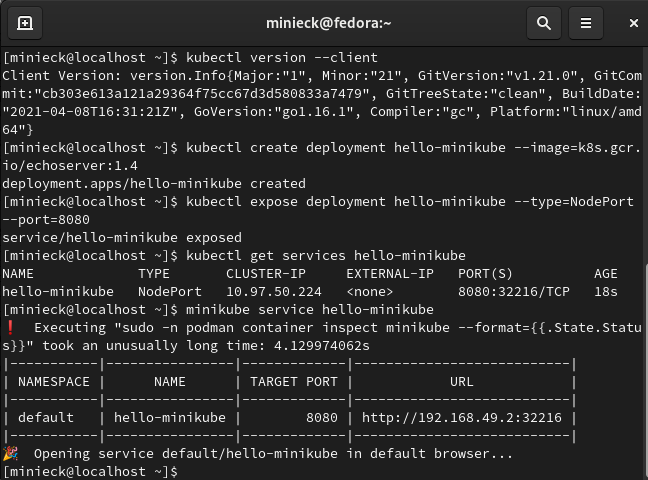
\includegraphics[width=\linewidth]{img/hellokube.png}
    \label{fig:hellokube}
    \caption[Het opstarten van een contianer met kubectl]{Met kubernetes is een container deployment aangemaakt.}
    \centering
\end{figure}

Om te werken met Kubernetes is er een dashboard weergave die met Minikube opgestart kan worden.
\begin{verbatim}
minikube dashboard
\end{verbatim}
Met deze dashboard kunnen veel van de functionaliteiten van Kubernetes gedaan worden zonder de CLI te gebruiken. zo is er via de dasboard een extra pod van de hello minikube container gestart zoals getoont in afbeelding \ref{fig:kubenetesDash}. Iets dat ook bijzonder interessant lijkt is dat bij het maken van een container in de dashboard met een form kan worden gewerkt. Hier is het voornaamste de naam in te stellen en een adres waarvan de image moet worden gepulled. Kubernetes heeft echter geen voor de hand liggende methode om lokaal bewaarde images of private images te gebruiken bij het starten van een container.
\begin{figure}[h]
    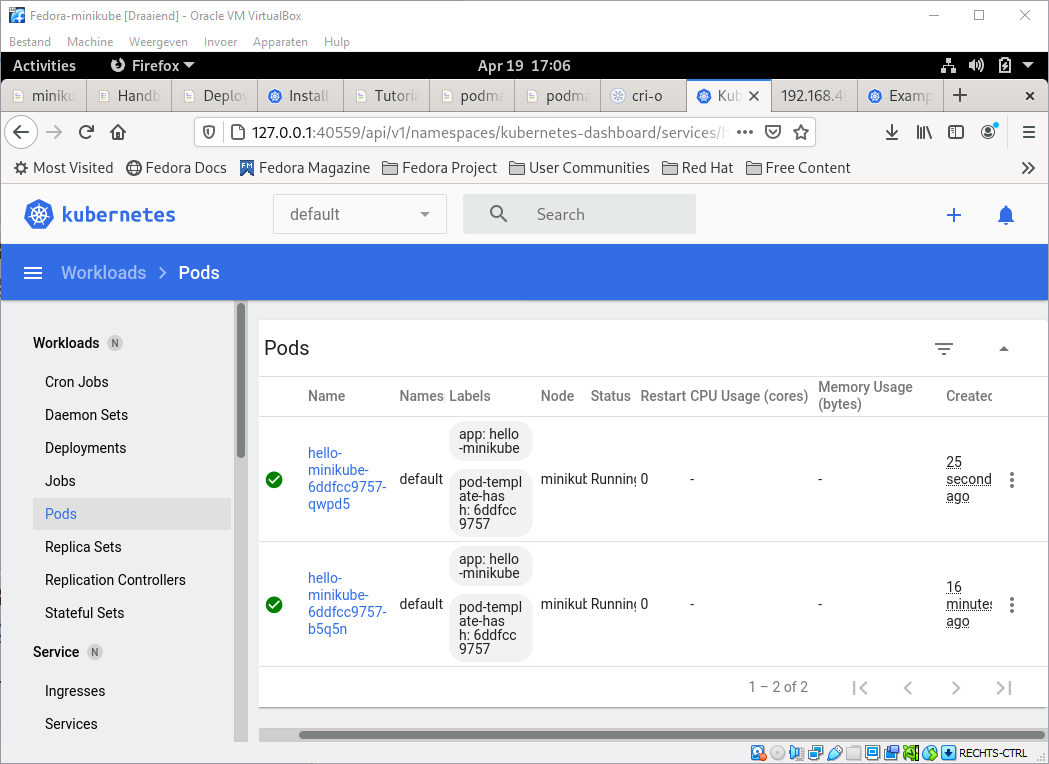
\includegraphics[width=\linewidth]{img/kubenetesDash.png}
    \label{fig:kubenetesDash}
    \caption[the kubenetes Dashboard]{hier toont de Kubernetes dashboard dat een nieuwe pod van de hellominikube container recent gestart is}
    \centering
\end{figure}
Vervolgens werd een op basis van een Kubernetes tutorial\footnote{\url{https://kubernetes.io/docs/tutorials/stateful-application/mysql-wordpress-persistent-volume/}}  een Wordpress site gemaakt. Dit gebeurt analoog als Docker compose met configuratie bestanden die door Kubernetes worden ingelezen. De configuratiebestanden voor de SQL-databank container en de wordpress container staan in bijlage 1 en 2. Het primaire bestand dat Kubernetes zal inlezen is een kustomization.yaml. Omdat het wachtwoord gevoelig is kan er gewerkt worden met een secret generator in de kustomization.yaml, dit is te zien in listing \ref{lst:kustomization} . Ook zijn de verwijzingen naar de configuratie van de resources voor de wordpress site toegevoegd aan dit bestand.
\begin{lstlisting}[caption=inhoud van kustomization.yaml,label=lst:kustomization]
secretGenerator:
- name: mysql-pass
literals:
- password=k8press
resources:
- mysql-deployment.yaml
- wordpress-deployment.yaml
\end{lstlisting}

Eens de kustomization.yml geconfigureerd is kan volgend commando worden uitgevoerd in de map met de 3 bestanden.
\begin{verbatim}
kubectl apply -k ./
\end{verbatim}
Om te controleren of dat het opstarten gelukt is kan gekeken worden via het dashboard van Kubernetes of met volgende commando’s:
\begin{verbatim}
kubectl get secrets
kubectl get pvc
kubectl get pods
kubectl get services wordpress
\end{verbatim}
Om effectief de wordpress site te kunnen bezoeken moet deze nog blootgesteld worden naar buiten de cluster. Hiervoor moet Minikube worde gebruikt:
\begin{verbatim}
minikube service wordpress –url
\end{verbatim}
met de teruggegeven URL kan de wordpress site in een browser worden bezocht om zo de installatie te beginnen.
Om de site weer te stoppen kan in de folder met de Kustomisation.yml volgend commando worden uitgevoerd om alles te stoppen en verwijderen.
\begin{verbatim}
kubectl delete -k ./
\end{verbatim}

om effectief te Kubernetes cluster te stoppen moeten moet het volgende commando worden uitgevoerd met minikube
\begin{verbatim}
minikube stop
\end{verbatim}

\paragraph{Ervaring}
Podman met GitHub container registry was zeer makkelijk en was zoals vermeld volledig analoog aan de Docker methode. De blogpost gaf een korte uitleg over hoe een container file verder aangepast kan worden om bepaalde zaken te configureren. Jammer genoeg lukte Buildah niet door een conflict tijdens de installatie met de al geïnstalleerde Podman. Buildah zou ook enkel nodig zijn om vanaf nul een nieuwe image te maken en zo zou podman woldoende zijn als er altijd een bestaande image als vertkerlpunt wordt gebruikt.

Het starten van Minikube met Podman vergt wat meer configuratie maar is niet onredelijk. Het gebruikt veel emoticons om berichten te accentueren wat afhankelijk van persoonlijke smaak een minpunt kan zijn. Eens de Minikube Kubernetes gestart is merk je niet meer waarop het effectief draait. Ook is Minikube licht genoeg om zonder problemen te werken met 4 GB ram, iets wat de Docker desktop Kubernetes niet kon.

Kubernetes zelf is zeer goed. Er zijn veel voorbeelden voor te vinden en werkt binnen Minikube. De Dashboard van Kubernetes is ook een zeer grote pluspunt. Het laat een gebruiker toe om de volledige cluster te beheren zonder noodzakelijk via de commandolijn te werken. Ook toont het bij het kiezen van een actie met het dashboard wat de equivalente commando zou zijn om het via command line te doen.


\subsection{Docker engine voor Nomad}
Hiervoor weer de Ubuntu deels om te zien of dat het installeren van Docker zou lukken en omdat deze verder al aan alle eisen voor Nomad voldeed.
\paragraph{Installatie en set-up}
De Docker engine installeren en opstarten lukt zonder problemen. Ook het installeren van Nomad zelf gaf geen complicaties.
\paragraph{Ingebruikname}
Na het installeren van de Docker engine werd er eerst getest of dat alles werkte zoals met Docker direct op de laptop lukte in sectie. Hierbij werden geen problemen ondervonden.

Hashi Corp heeft een korte tutorial\footnote{\url{https://learn.hashicorp.com/collections/nomad/get-started}} die een inleiding geeft tot het werken met Nomad. Eerst moet de lokale agent voor Nomad worden gestart.
\begin{verbatim}
sudo nomad agent -dev -bind 0.0.0.0 -log-level INFO
\end{verbatim}
Eens Nomad gestart is kan in en nieuwe terminal met de agent worden gewerkt. Eerst stel de tutorial voor om status en member op te halen aan de hand van
\begin{verbatim}
nomad node status
\end{verbatim}
en
\begin{verbatim}
nomad server members
\end{verbatim}

Voor het werken met de jobs die Nomad hanteert stel hasicorp voor om te vertrekken met het volgend commando om in de huidig actieve map een exmaple.nomad te genereren de inhoud woord ook getoont in bijlage. Dit is een kleine container van een redis image die met de docker engine wordt uitgevoerd
\begin{verbatim}
nomad job init
\end{verbatim}
Om deze nieuwe job effectief te starten moet volgend commando worden uitgevoerd en word getoont in figuur \ref{fig:nomadrun}.
\begin{verbatim}
nomad job run example.nomad
\end{verbatim}
de naam die Nomad geeft aan de job eens deze gestart is, is het deel voor de ‘.nomad’ zo kan de status van het voorbeeld worden opgehaald met
\begin{verbatim}
nomad job status example
\end{verbatim}
Om aan te passen hoeveel instanties van de redis container draaien moet eerst het job bestand worden aangepast. Hiervoor moet op lijn 143 in example.nomad het volgende komen te staan
\begin{verbatim}
# The "count" parameter specifies the number of the task groups that should
# be running under this group. This value must be non-negative and defaults
# to 1.
+ count = 3
\end{verbatim}
Op de huidig actieve job te doen updaten met de nieuwe vereisten moet de verandering ingeplant worden in de scheduler van Nomad
\begin{verbatim}
nomad job plan example.nomad
\end{verbatim}
Als output van dit commando wordt de job modify index meegegeven om vervolgen de aanpassing door te voeren moet deze worden uitgevoerd aan de hand van
\begin{verbatim}
nomad job run -check-index 16 example.nomad.
\end{verbatim}
Een andere update wordt ook uitgelegd in de tutorial hiervoor wordt de redis versie in het bestand op lijn 305 aangepast naar image = "redis:4.0". Analoog moet deze aanpassing eerst geplant worden en vervolgen uitgevoerd.
Met de dev agent die gestart is wordt een web interface voorzien op http://localhost:4646. Met de web interface kan je de huidige status van de Nomad cluster raadplegen. Echter om iets aan te passen moet gewerkt worden met een job bestand dat in deze in deze interface kan worden geplakt zoals te zien in figuur \ref{fig:nomdaddash}.

Door de bijkomende barrière van de hasiorp configuration language is het niet gelukt om een wordpress site te starten met Nomad.

Na het installeren van de Docker engine werd er eerst getest of dat alles  werkte zoals het direct op de laptop lukte. Hierbij werden geen problemen ondervonden. Hierna werd een dev omgeving Nomad instantie opgestart om eens mee te werken.
\begin{figure}[h]
    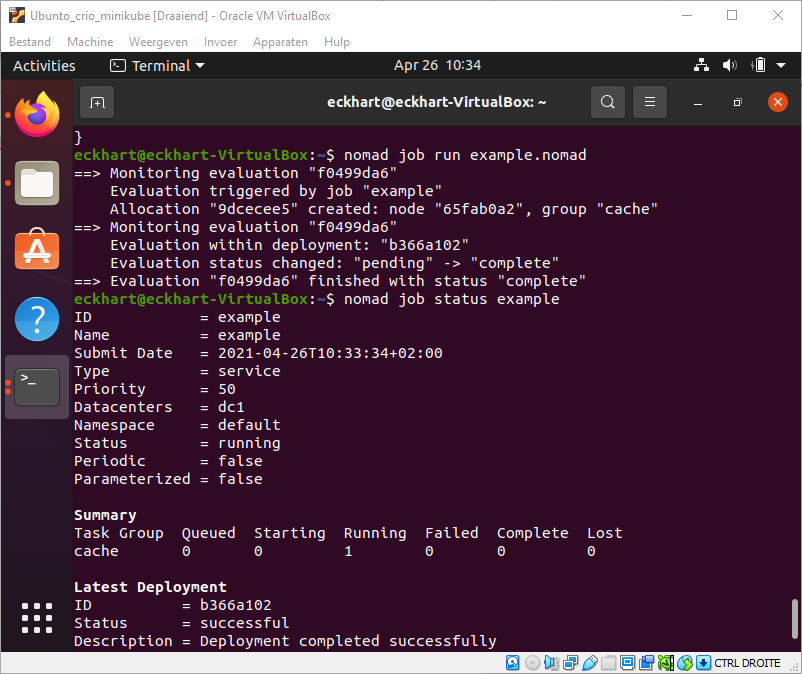
\includegraphics[width=\linewidth]{img/nomadrun.png}
    \label{fig:nomadrun}
    \caption[Een voorbeeld Nomad job]{hier wordt via de cli van Nomad de example.nomad job gestart}
    \centering
\end{figure}
\begin{figure}[h]
    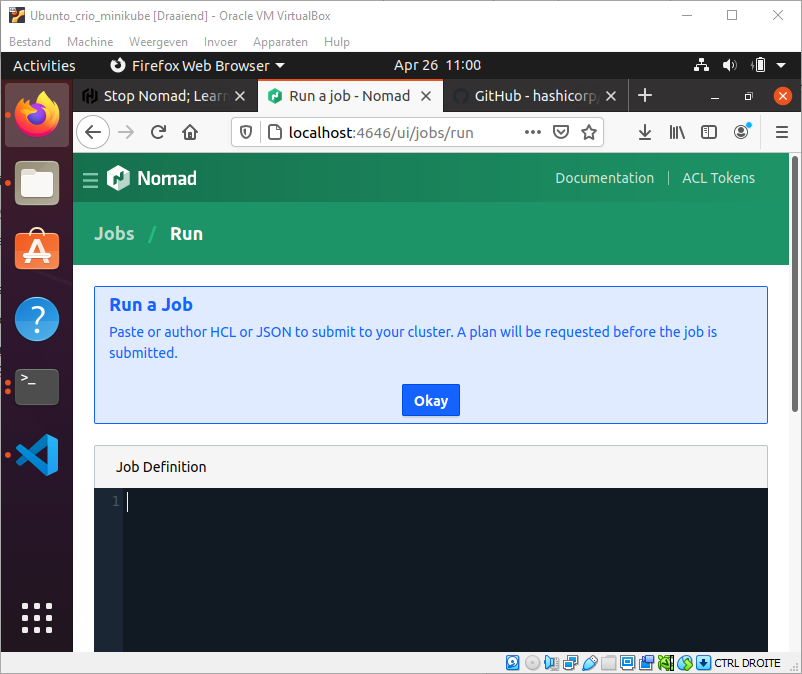
\includegraphics[width=\linewidth]{img/nomdaddash.png}
    \label{fig:nomdaddash}
    \caption[de nomad dashboard]{de dashboard weergave om een job te starten met Nomad}
    \centering
\end{figure}


\paragraph{Ervaring}
Door Nomad werking met jobs voor alle taken is er een duidelijk verschil met Kubernetes. Een groot voordeel is dat Nomad meer kan beheren dan enkel containers. Maar het heeft zeker zijn minpunten. Zo is de eigen markup voor de configuratie een bijkomende barrière voor het werken met Nomad in vergelijking met de al veelgebruikte YAML die Docker, Podman en Kubernetes allemaal gebruiken.  Visual studio code heeft gelukkig een extensie voor de Configuratie Taal die hashicorp gebruikt die het werken met deze .Nomad  bestanden helpt. Nomad heeft ook een web browser gebaseerde interface maar deze toont niet wat een equivalent commando voor de command line zou zijn. Het is ook in het algemeen minder gebruikt dan Kubernetes waardoor uitleg en integratie minder is.  

\section{Samengevatte resultaten software Tests}
%% TODO: insert table comarisons?
Dit deel vergelijkt samengevat eens de technologieën die gebruikt zijn. Enkel voor orchestration is er een duidelijke voorkeur voor Kubernetes als leermiddel.

\subsection{Runtimes}

In basis gebruik lijken Docker en Podman goed op elkaar. De grootste verschillen zitten in de installatie en de eigen werking voor meerdere samenhangende containers. Qua installatie komt Podman standaard geïnstalleerd in Fedora, en moet Docker altijd geïnstalleerd worden. De Docker compose die afhankelijk afzonderlijk geïnstalleerd moet worden maakt het verbinden van container mogelijk  Het equivalent in Podman met de pods is iets complexer en zelfs met een extra overbrugging van Podman Compose niet voor de hand liggend. Echter deze verbinding tussen container kan ook gedaan worden in Kubernetes en is bij gebruik van Kubernetes niet meer zo belangrijk.

Verder is de Docker desktop voor het leren maar een kleine meerwaarde. Het is ten eerste niet beschikbaar op linux systemen. Ten tweede moeten veel functionaliteiten nog via de command line uitgevoerd worden. De desktop applicatie een overzicht van lokale images het maken van een nieuwe image moet via command line interface. Ten derde is de gebundelde Kubernetes zwaarder dan een Kubernetes instantie met Minikube.

\subsection{Repositories}

Tussen de twee gebruikte repository is er niet meteen een de beter is dan de andere. De Docker hub wordt door zowel Docker als Podman gebruikt als standaard doel om image te pushen. Dit beteken dat er weinig aangepast moet worden om effectief te pushen of pullen. Echter de Docker hub zet standaard images publiek en heeft maar een private image mogelijkheid voor gratis accounts. De GitHub container registry daarentegen zou een beetje extra werk vragen om het doel voor het pushen van een image te selecteren. Het zou wel geen extra account nodigen hebben als de student al reeds met GitHub werkt. Over de specifieke kosten en regeling van de GitHub container registry kan er nog geen uitspraak gedaan worden doordat deze nog in bèta fase is. Zou het zelfde limiet  van 500 mb voor private containers gelden als op de rest van GitHub packages zou deze te klein zijn om meer te beteken dan één of enkele private images.

\subsection{Orchestration}

Voor orchestration is Kubernetes de beste van de twee geteste voor het werken met containers. Zo heeft het een dashboard weergave die niet alleen de noodzaak voor het werken via command line minimaliseert, het toont ook bij het uitvoeren van taken via deze dasboard de equivalente commando’s om het via cli te doen. Om met Kubernetes te leren werken is de beschikbaarheid Minikube ook een pluspunt. Minikube helpt om een lokale Kubernetes cluster op te starten en beheren. Verder kan Minikube ook de juiste verbindingen maken om een keuze aan achterliggende runtime te hebben.  Minikube heeft de beste ondersteuning voor Docker als engine maar kan met wat extra configuratie een het installeren kan Cri-o als hulpstuk ook met Podman als runtime werken. één van de grotere minpunten die eigen is aan Kubernetes is dat het moeilijk is om containers te draaien op basis van lokaal bewaarde images of privé bewaard in een repository.

Om specifiek met containers te werken is Nomad minder aan te raden. De hasicorp configuration language is ook een extra stap in het leerproces. Het kan dat een student Yaml dei Kubernetes gebruikt nog niet gezien heeft, maar de kans is groter dat de student ook Yaml elders zal tegenkomen dan de Hasicorp markup. Ook iets dat het leren ten nadele zou komen ten opzichte van Kubernetes is dat de dashboard niet de equivalente commando’s toont, dit is deels toe te kennen aan de methodologie van Nomad om aanpassingen aan je draaiende containers te doen op basis van jobs, die telkens geschreven moeten worden in de hasicorp configuration language.
